%!TEX root=Principal.tex
\chapter{CRONOGRAMA}
\label{cap:cronograma}
Nesse capitulo é apresentado o cronograma definido para a conclusão da tese. O início do cronograma é demarcado a partir da apresentação do exame de qualificação, conforme apresentado na figura~\ref{fig:cronograma}.

\begin{figure}[ht!]
	\centering
	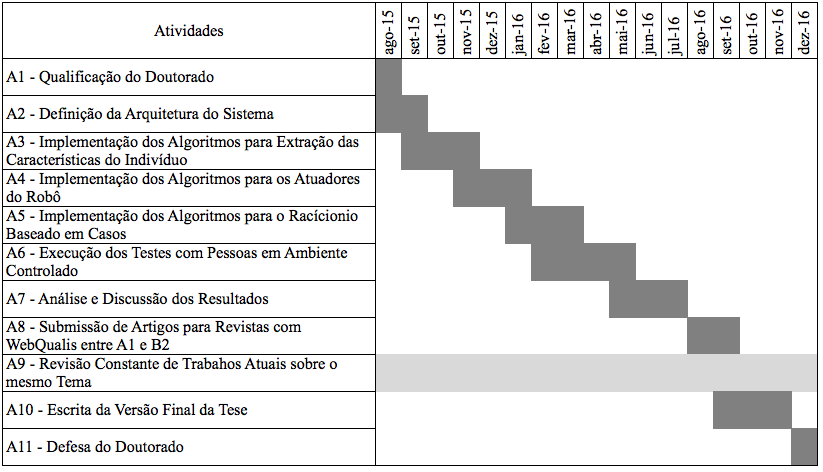
\includegraphics[width=\textwidth]{images/cronograma.png}
	\caption{Cronograma para Conclusão da Tese.}
	\label{fig:cronograma}
\end{figure}

A lista a seguir apresenta com mais detalhes as tarefas apresentadas no cronograma da figura~\ref{fig:cronograma}.

\begin{enumerate}
	\item \textbf{A1}: Apresentação do Exame de Qualificação para o Doutorado;
	\item \textbf{A2}: Definição da Arquitetura que irá auxiliar o desenvolvimento e execução do Sistema que poderá ser consumido por diferentes tipos de robô ao mesmo tempo;
	\item \textbf{A3}: Desenvolvimento dos algoritmos que serão utilizados para fazer com que o robô possa extrair as informações comportamentais das pessoas, de acordo com o apresentado na seção~\ref{sec:extracaocaracteristicas};
	\item \textbf{A4}: Desenvolvimento dos algoritmos que irão controlar os atuadores do robô, como por exemplo, cabeça, manipulador e motores;
	\item \textbf{A5}: Desenvolvimento dos algoritmos que compõem o mecanismo para Raciocínio Baseado em Casos, responsável pelo aprendizado de interação do robô;
	\item \textbf{A6}: Execução dos testes de interação de acordo com o descrito no capitulo~\ref{cap:testes};
	\item \textbf{A7}: Análise dos resultados utilizando métodos estatísticos e também as observações obtidas durante o acompanhamento dos testes de interação;
	\item \textbf{A8}: Submissão de pelo menos 2 artigos sobre a tese para revistas relevantes para a área de pesquisa, classificadas de acordo com o WebQualis da CAPES entre os níveis de A1 à B2;
	\item \textbf{A9}: Revisão bibliográfica contínua para certificar da originalidade e atualidade do trabalho de tal forma, que sua contribuição possa ajudar o avanço da área de pesquisa em robótica social e assistiva;
	\item \textbf{A10}: Consolidação do trabalho no texto do documento da tese para entrega à banca avaliadora;
	\item \textbf{A11}: Apresentação da Defesa para o título de Doutor.
\end{enumerate}